\documentclass[compress]{beamer}        % [compress] (written before {beamer} <=> navigation bar one line, all subsections in 1 line instead of 2

% Setup appearance:
\usetheme{CambridgeUS}
%	AnnArbor | Antibes | Bergen |
%	Berkeley | Berlin | Boadilla |
%	boxes | CambridgeUS | Copenhagen |
%	Darmstadt | default | Dresden |
%	Frankfurt | Goettingen |Hannover |
%	Ilmenau | JuanLesPins | Luebeck |
%	Madrid | Malmoe | Marburg |
%	Montpellier | PaloAlto | Pittsburgh |
%	Rochester | Singapore | Szeged |
%	Warsaw
%

\useoutertheme[footline=authorinstitute,subsection=false]{miniframes}
\usecolortheme{whale}

%	albatross | beaver | beetle |
%	crane | default | dolphin |
%	dove | fly | lily | orchid |
%	rose |seagull | seahorse |
%	sidebartab | structure |
%	whale | wolverine


\setbeamertemplate{footline}
{
  \hbox{%
  \begin{beamercolorbox}[wd=.25\paperwidth,ht=2.25ex,dp=1ex,center]{title in head/foot}%
    \usebeamerfont{date in head/foot}\insertshortauthor
  \end{beamercolorbox}%
  \begin{beamercolorbox}[wd=.5\paperwidth,ht=2.25ex,dp=1ex,center]{date in head/foot}%
    \usebeamerfont{title in head/foot}\insertshortinstitute
  \end{beamercolorbox}%
  \begin{beamercolorbox}[wd=.25\paperwidth,ht=2.25ex,dp=1ex,center]{title in head/foot}%
    \usebeamerfont{date in head/foot}
    \insertframenumber{} / \inserttotalframenumber
    %\insertframenumber{} / \insertpresentationendpage
  \end{beamercolorbox}}%
  \vskip0pt%
}

%\setbeamercolor{titlelike}{parent=structure}
%\setbeamercolor{structure}{fg=beamer@blendedblue}
%% \useinnertheme{rounded}
%\setbeamerfont{block title}{size={}}
%\usefonttheme[onlylarge]{structurebold}   % title and words in the table of contents bold
%\setbeamerfont*{frametitle}{size=\normalsize,series=\bfseries}
\setbeamertemplate{navigation symbols}{}
\setbeamercolor{frametitle}{parent=boxes, bg=white}
{ % only on titlepage


\usepackage{times}
\usepackage{amsmath,amssymb,amsthm}
\usepackage{color}
\usepackage{changepage}
\usepackage{multirow}
\usepackage[absolute,overlay]{textpos}
\usepackage{enumerate}
%\usepackage{pgfpages}
\usepackage[all]{xy}
\usepackage{textcomp}
\usepackage{etex}
\usepackage{tikz}
\usetikzlibrary{shapes}
%\usepackage{handoutWithNotes}
%\pgfpagesuselayout{4 on 1}[border shrink=1mm]




\definecolor{camblue}{RGB}{26,26,89}
\definecolor{Rblue}{RGB}{0,255,255}
\definecolor{Rdarkblue}{RGB}{0,0,255}
\definecolor{Rgreen}{RGB}{0,205,0}
\definecolor{green2}{RGB}{51,204,51}
\newcommand{\tcb}{\textcolor{beamer@blendedblue}}
\newcommand{\tcbb}{\textcolor{camblue}}
\newcommand{\tcr}{\textcolor{red}}
\newcommand{\tcg}{\textcolor{gray}}
\newcommand{\tcgr}{\textcolor{green2}}
\newcommand{\tcblk}{\textcolor{black}}
\newcommand{\tcRg}{\textcolor{Rgreen}}
\newcommand{\tcRdb}{\textcolor{Rdarkblue}}
\newcommand{\tcRb}{\textcolor{Rblue}}
\newcommand{\tcw}{\textcolor{white}}
\newcommand{\m}{\phantom{-}}
\newcommand{\bp}{\tcbb{$\bullet$}\:}


\title{{\huge Statistics for Computing\\[0.1cm]MA4413}}
\author[Kevin Burke]{{\bf\\[0.5cm]{\huge Lecture 11}\\[0.2cm]\emph{Sum / Difference of Independent Normal Variables and\\Calculating Normal Limits}\\[1.4cm]Kevin Burke}\\[0.3cm]\tcb{kevin.burke@ul.ie}}

\institute[University of Limerick, Maths \& Stats Dept]{}
\date{}

%\TPGrid[5mm,5mm]{1}{1}

\begin{document}


\begin{frame}[t]
\titlepage
\end{frame}



\section{Sum / Difference of Normal Variables}
\subsection{Sum / Difference of Normal Variables}
\begin{frame}{\bf \tcb{Sum / Difference of Normal Variables}}

If $X_1 \sim \text{Normal}(\mu_1,\sigma_1)$ and $X_2 \sim \text{Normal}(\mu_2,\sigma_2)$ are {\bf independent normal variables} then the {\bf sum} is\\
\begin{align*}
\boxed{X_1 + X_2 \sim \text{Normal}(\mu = \mu_1+ \mu_2,\,\, \sigma = \sqrt{\sigma_1^2+\sigma_2^2}\,)},\\
\end{align*}
and the {\bf difference} is\\
\begin{align*}
\boxed{X_1 - X_2 \sim \text{Normal}(\mu = \mu_1 - \mu_2,\,\, \sigma = \sqrt{\sigma_1^2+\sigma_2^2}\,)}.\\
\end{align*}

Note that in \emph{both} cases $\sigma = \sqrt{\sigma_1^2+\sigma_2^2}$.


\end{frame}



\subsection{Example: Batteries}
\begin{frame}{\bf \tcb{Example: Batteries}}

Let the voltages for two batteries be $X_1 \sim \text{Normal}(\mu_1=6,\sigma_1=0.1)$ and $X_2 \sim \text{Normal}(\mu_2=6,\sigma_2=0.1)$ where $X_1$ and $X_2$ are independent.\\[0.5cm]

Let's assume that a 12V battery is made up of two of these batteries. Let $Y$ represents the total voltage:
\begin{align*}
Y = X_1 + X_2 &\sim \text{Normal}(\mu = 6+ 6,\,\, \sigma = \sqrt{0.1^2+0.1^2}\,)\\[0.2cm]
&\sim \text{Normal}(\mu = 12,\,\, \sigma = 0.1414).\\
\end{align*}

We can then calculate probabilities as before, e.g.,
\begin{align*}
\Pr(Y > 12.15) = \Pr(Z > \tfrac{12.15-12}{0.1414}) = \Pr(Z > 1.06) = 0.1446.
\end{align*}



\end{frame}




\subsection{Question 1}
\begin{frame}{\bf \tcb{Question 1}}

Let $X_1$ represent the time it takes a person to complete a particular task where $X_1 \sim \text{Normal}(\mu=45,\sigma=1)$. Another individual's time is $X_2 \sim \text{Normal}(\mu=44,\sigma=1.5)$. Let $Y = X_1 - X_2$.\\[0.2cm]

\begin{enumerate}[a)]\itemsep0.3cm
\item What is the distribution of $Y$?
\item What is the probability that person 1 finishes first?
\item What is the probability that person 2 finishes first?
\item What is the probability that the winner finishes at least 2 seconds before the other person?
\end{enumerate}


\end{frame}



\section{Normal Limits}
\subsection{95\% Limits}
\begin{frame}{\bf \tcb{95\% Limits}}

For a variable $X \sim \text{Normal}(\mu,\sigma)$, it is often of interest to calculate {\bf limits} $x_1$ and $x_2$ such that

\begin{align*}
\Pr(x_1 < X < x_2) = 0.95.\\
\end{align*}

More specifically, this interval is constructed to cover the {\bf central 95\%} of the distribution.\\[0.7cm]

Thus 5\% of the distribution remains:\\[0.1cm]
\begin{itemize}\itemsep0.3cm
\item 2.5\% in the lower tail (below $x_1$)
\item 2.5\% in the upper tail (above $x_2$)
\end{itemize}

\end{frame}


\subsection{95\% Limits}
\begin{frame}{\bf \tcb{95\% Limits}}

\begin{center}
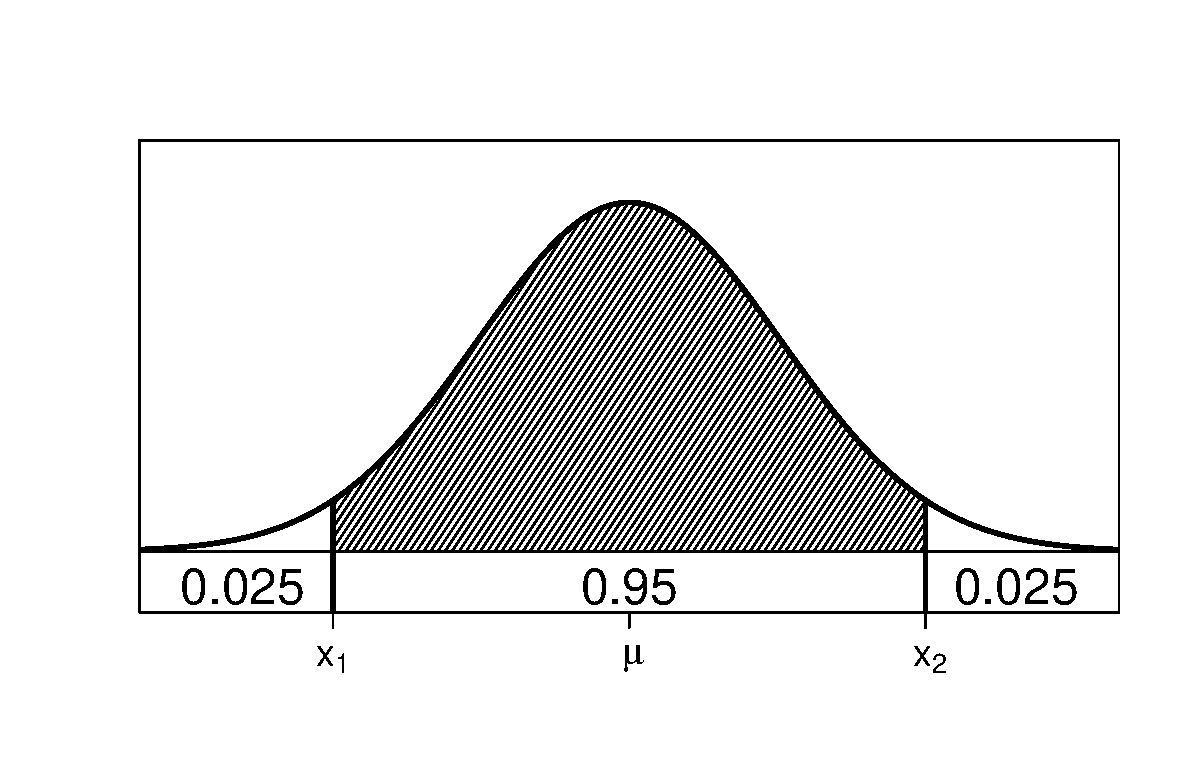
\includegraphics[width=0.98\textwidth, trim = 1.5cm 1.5cm 0.7cm 1.5cm, clip]{Norm95}
\end{center}

\end{frame}



\subsection{Example: Salary}
\begin{frame}{\bf \tcb{Example: Salary}}

We return to the salary example from the previous lecture where $X \sim \text{Normal}(\mu=30,\sigma=4)$.\\[0.5cm]

We will now calculate the 95\% salary limits:
\begin{align*}
\text{{\bf lower}}&\text{{\bf \,\,tail}}  & \text{{\bf upper}}&\text{{\bf \,\,tail}} \\[0.2cm]
\Pr(X < x_1) &= 0.025 & \Pr(X > x_2) &= 0.025\\[0.2cm]
\Pr(Z < \tfrac{x_1-30}{4}) &= 0.025 & \Pr(Z > \tfrac{x_2-30}{4}) &= 0.025 \\[0.2cm]
\Pr(Z > -\tfrac{x_1-30}{4}) &= 0.025 &&\\[-0.3cm]
\end{align*}

We find that the $z$ score which corresponds to $\Pr(Z > z) = 0.025$ is $z = 1.96$ (from the tables).

\begin{textblock}{1}(8.25,7.5)
\xymatrixcolsep{0.8cm}
\rule{1pt}{2.7cm}
\end{textblock}

\end{frame}


\subsection{Example: Salary}
\begin{frame}{\bf \tcb{Example: Salary\\[-1.1cm]}}\label{salary95int}

\begin{align*}
\text{{\bf lower}}&\text{{\bf \,\,limit}}  & \text{{\bf upper}}&\text{{\bf \,\,limit}} \\[0.2cm]
-\tfrac{x_1-30}{4} &= 1.96 & \tfrac{x_2-30}{4} &= 1.96 \\[0.2cm]
\tfrac{x_1-30}{4} &= -1.96 && \\[0.2cm]
x_1-30 &= -1.96(4) & x_2-30 &= 1.96(4) \\[0.2cm]
x_1 &= 30 - 1.96(4) & x_2 &= 30 + 1.96(4) \\[0.2cm]
x_1 &= 22.16 & x_2 &= 37.84 \\[0.2cm]
\end{align*}

In words, the central 95\% of salaries lie in the interval $[22.16,\,\, 37.84]$.\\[0.5cm]

Note: this interval can be written $30 \pm (1.96\times4)$. \,\,\emph{(more on this later)}

\begin{textblock}{1}(8.1,3.2)
\xymatrixcolsep{0.8cm}
\rule{1pt}{5cm}
\end{textblock}

\end{frame}


\subsection{Example: Salary}
\begin{frame}{\bf \tcb{Example: Salary}}

\begin{center}
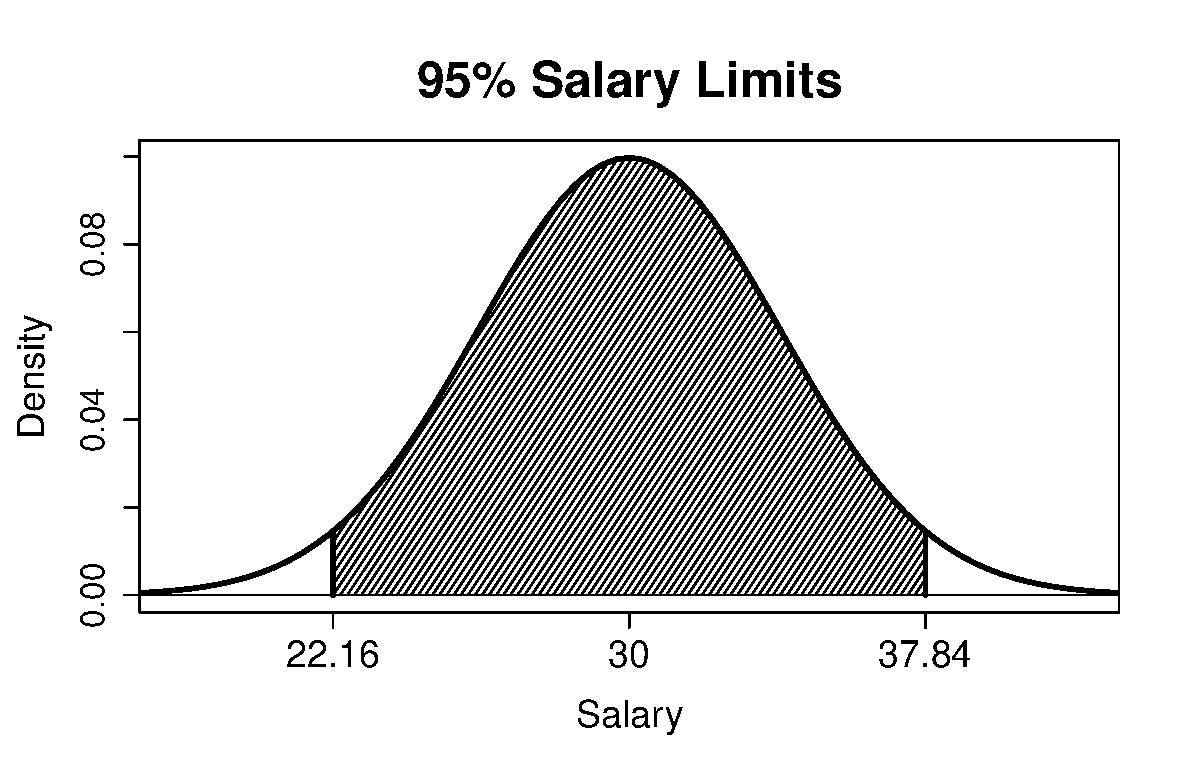
\includegraphics[width=0.98\textwidth, trim = 0.0cm 0.5cm 0.3cm 0.5cm, clip]{Norm95Salary}
\end{center}

\end{frame}

\subsection{$(1-\alpha)100\%$ Limits}
\begin{frame}{\bf \tcb{$(1-\alpha)100\%$ Limits}}

We can calculate the limits for other percentage values:\\[0.1cm]

\begin{align*}
\Pr(x_1 < X < x_2) = 1-\alpha,\\[-0.0cm]
\end{align*}

where $x_1$ and $x_2$ are chosen so that the central probability of $1-\alpha$ is covered ($\alpha$ is the Greek letter ``alpha'').\\[0.5cm]

Thus the probability $\alpha$ remains:\\[0.1cm]
\begin{itemize}\itemsep0.3cm
\item $\alpha/2$ in the lower tail (below $x_1$)
\item $\alpha/2$ in the upper tail (above $x_2$)\\[0.5cm]
\end{itemize}

Example: $\alpha=0.01$ $\Rightarrow$ $(1-0.01)\times100\% = 99\%$ limits with $\alpha/2 = 0.005$ remaining in each tail (i.e., 0.5\%).

\end{frame}


\subsection{$(1-\alpha)100\%$ Limits}
\begin{frame}{\bf \tcb{$(1-\alpha)100\%$ Limits}}

\begin{center}
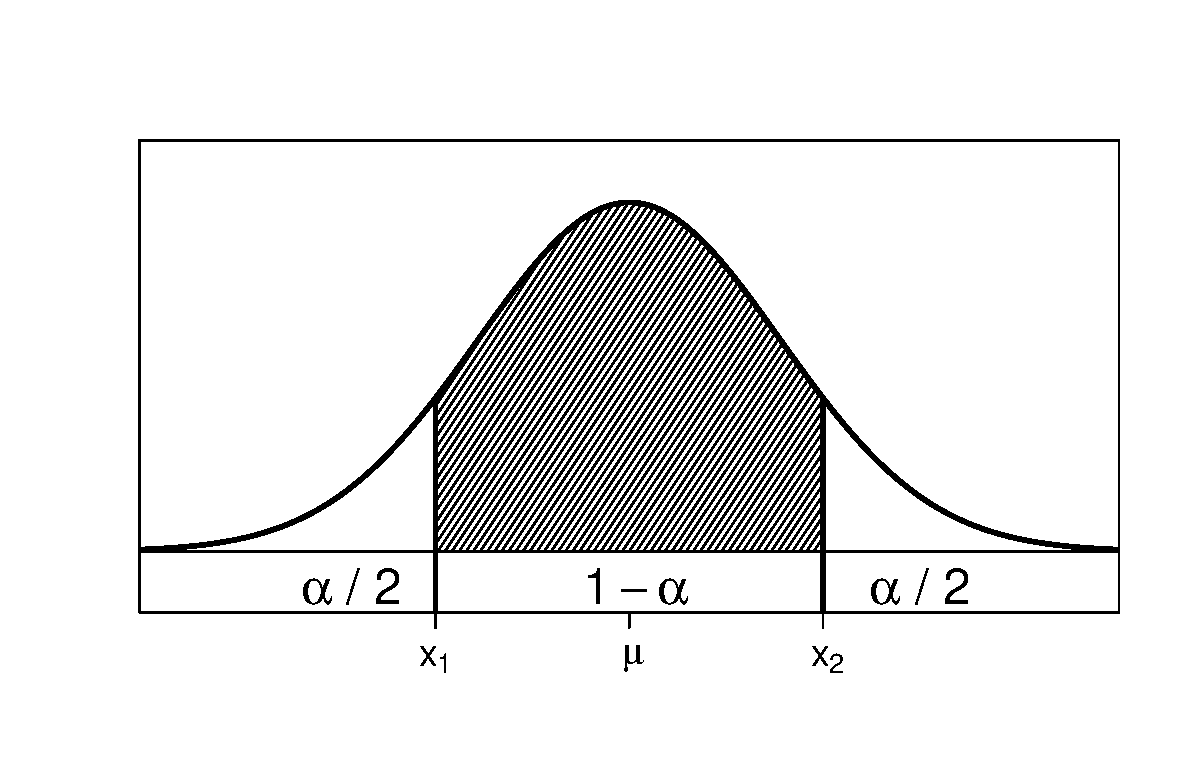
\includegraphics[width=0.98\textwidth, trim = 1.5cm 1.5cm 0.7cm 1.5cm, clip]{NormAlpha}
\end{center}

\end{frame}


\subsection{Question 2}
\begin{frame}{\bf \tcb{Question 2}}

We continue with salary $X \sim \text{Normal}(\mu=30,\sigma=4)$.\\[0.2cm]

\begin{enumerate}[a)]
\item Calculate the limits within which the central 99\% of salaries lie.
\end{enumerate}


\end{frame}


\section{Constructing Limits}
\subsection{Example: Salary}
\begin{frame}{\bf \tcb{Example: Salary}}

We noted that the 95\% salary limits can be written in the form:
\begin{align*}
30 \pm (1.96\times4)
\end{align*}
We now let $z_{\,0.025} = 1.96$ since it is the $z$ score corresponding to a probability of $0.025$ in the tables, i.e., $\Pr(Z > 1.96) = 0.025$.\\[0.3cm]
Thus, the 95\% limits are:\\[-0.7cm]
\begin{align*}
30\pm (z_{\,0.025}\times4)
\end{align*}

Similarly, the 99\% limits are:\\[-0.7cm]
\begin{align*}
30\pm (z_{\,0.005}\times4)
\end{align*}

$\Rightarrow$ The $(1-\alpha)100\%$ limits are:\\[-0.7cm]
\begin{align*}
30\pm (z_{\,\alpha/2}\times4)
\end{align*}

\end{frame}

\subsection{Constructing Limits}
\begin{frame}{\bf \tcb{Constructing Limits}}

For a general Normal$(\mu,\sigma)$ distribution, the interval\\
\begin{align*}
\boxed{\mu \, \pm \, z_{\,\alpha/2} \,\, \sigma}\\[-0.2cm]
\end{align*}
contains $(1-\alpha)100\%$ of the distribution. This fact can be stated\\[0.1cm] mathematically as $\Pr(\mu - z_{\,\alpha/2} \,\, \sigma < X < \mu + z_{\,\alpha/2} \,\, \sigma) = 1 - \alpha$.\\[0.7cm]

In practice, we do not need to go through the probability arguments of the previous slides every time.\\[0.7cm]

Simply look up the $z_{\,\alpha/2}$ score in the tables and use the above formula.

\end{frame}


\subsection{Commonly Used Limits}
\begin{frame}{\bf \tcb{Commonly Used Limits}}

It is very common to compute the following:\\
\begin{center}
\begin{tabular}{|cccc|}
\hline
&&&\\[-0.3cm]
\% & $\alpha$ & $z_{\,\alpha/2}$ & Interval \\[0.1cm]
\hline
&&&\\[-0.3cm]
90\% & 0.10 & $z_{\,0.05} =1.64$ & $\mu \pm 1.64 \, \sigma$\\[0.4cm]
95\% & 0.05 & $z_{\,0.025} =1.96$ & $\mu \pm 1.96 \, \sigma$\\[0.4cm]
99\% & 0.01 & $z_{\,0.005} =2.58$ & $\mu \pm 2.58 \, \sigma$\\[0.1cm]
\hline
\multicolumn{4}{c}{}
\end{tabular}
\end{center}

Of course, any interval can be calculated, e.g., $\mu \pm 1.28 \, \sigma$ gives the 80\% limits, $\mu \pm 0.67 \sigma$ gives the 50\% limits etc.

\end{frame}




\subsection{R Code}
\begin{frame}{\bf \tcb{R Code}}
We can look up $z_{\,\alpha/2}$ scores in the normal tables. We can also do this using \texttt{qnorm}:\\[0.3cm]

\begin{tabular}{|l|}
\hline
Examples: \\[0.2cm]
\texttt{qnorm(0.05,mean=0,sd=1,lower=F)} \\
gives \texttt{1.644854}.\\[0.2cm]
\texttt{qnorm(0.025,mean=0,sd=1,lower=F)} \\
gives \texttt{1.959964}.\\[0.2cm]
\texttt{qnorm(0.005,mean=0,sd=1,lower=F)} \\
gives \texttt{2.575829}.\\[0.2cm]
\hline
\multicolumn{1}{c}{}\\[0.0cm]
\end{tabular}

Compare the above to the previous slide.

\end{frame}



\subsection{R Code}
\begin{frame}{\bf \tcb{R Code}}
Note that we can also construct the intervals directly using \texttt{qnorm}:\\[0.3cm]

\begin{tabular}{|l|}
\hline
Examples: \\[0.2cm]
\texttt{qnorm(0.025,mean=30,sd=4,lower=T)} \\
gives \texttt{22.16014}.\\[0.2cm]
\texttt{qnorm(0.025,mean=30,sd=4,lower=F)} \\
gives \texttt{37.83986}.\\[0.2cm]
\hline
\multicolumn{1}{c}{}\\[0.0cm]
\end{tabular}

Compare this with slide \pageref{salary95int}.


\end{frame}








\end{document} 